\chapter{Geographic View}
\label{sec:geo_view}

The Geographic View allows a graphical representation of target reports from the DBContent. After creation, it displays a world map in the map widget on the left, and a configuration panel on the right hand side.

\subfile{geo_layout}

\subfile{geo_toolbar}

\subfile{geo_data_widget}

\subfile{geo_config_panel}

\section{Import of GeoTIFF Files}

External GeoTIFF files can be imported into Geographic View by dragging and dropping them into Geographic Views map view.
If the import succeeds the imported grid data will be listed in the 'Layer' tab under \textit{Annotations}$\rightarrow$\textit{Grids}. 
Interaction with these items is explaned in section \ref{sec:geo_annotation_ops}. \\

Imported GeoTIFF files will persist until COMPASS is closed. \\

\begin{figure}[H]
  \center
    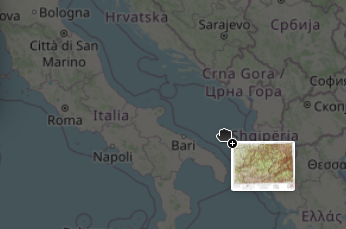
\includegraphics[width=12cm]{figures/geoview_import_geotiff.png}
  \caption{Import of a GeoTIFF file into Geographic View}
\end{figure}
